\section{VAR}

传统的自回归模型基于 next-token 预测,其 token 序列为简单的逐行排列,存在如下问题:
\begin{enumerate}
    \item 数学上的不符。编码器输出的 $\bm{z}_e(\bm{x})$ 其各位置的特征是相互依赖的,即
    $\bm{z}_q(\bm{x})$ 的 token 序列 $(x_1,x_2,\cdots)$ 之间存在双向关系,单向的自回归不适用;
    \item 单向的自回归预测限制了模型的泛化能力,如在双向依赖的问题中;
    \item 逐行排列的自回归结构破坏了图像固有的2D空间结构、依赖关系;
    \item 计算效率低。
\end{enumerate}
VAR 模型提出了基于 next-scale 预测的 multi-scale 自回归新范式,其预测方式符合天然的视觉特性,从模糊到清晰、从结构到细节,
VAR 具有类似于 LLMs 的优良特性:scaling laws 以及 zero-shot generalization;另外,VAR 的出现是自回归模型领域的突破,
在图像生成领域首次超过扩散模型(Diffusion Models)。

不同于 next-token 预测,VAR 基于 next-scale 预测,每个自回归单元为一整个图像 token,而不是单个位置的特征 token,
对于编码器的输出特征 $f\in\mathbb{R}^{h\times w\times C}$,其被量化为 $K$ 个 multi-scale 图像 token 序列
$(r_1,r_2,\cdots,r_K)$,其中分辨率 $h_k\times w_k$ 依次递增,直到 $r_K$ 对应原始大小 $h\times w$,自回归似然函数为:
\begin{equation}
    P(r_1,r_2,\cdots,r_K) = \prod_{k=1}^K P(r_k|r_{1},r_{2},\cdots,r_{k-1}),
\end{equation}
每个自回归单元 $r_k\in[V]^{h_k\times w_k}$,令 $Z$表示码本向量集,$V$表示其大小。在第 $k$ 步预测 $r_k$ 时,
$(r_1,r_2,\cdots,r_{k-1})$作为输入,采用 block-wise 因果注意力掩码。VAR 的这种自回归范式没有破坏图像的空间结构,
并且保持了天然的 $coarse-to-fine$ 的视觉特性,其次,其计算效率也大幅提高。VAR 自回归的具体范式如图~\ref{fig:VAR}所示,多尺度
图像 token 序列 $(r_1,r_2,\cdots,r_K)$ 由如下算法生成,其中 $r_k$ 对应码本中的索引矩阵,$z_k$ 为相应的量化特征向量,
$\hat{f}$ 为基于 $r_k$ 重构的特征向量,算法采用了残差范式,另外为避免扩展 $z_k$ 时的信息丢失,
采用了额外的 $K$ 个卷积层 $\{\phi_k\}_{k=1}^K$ 进行作用。

\begin{figure}[htbp]
    \centering 
    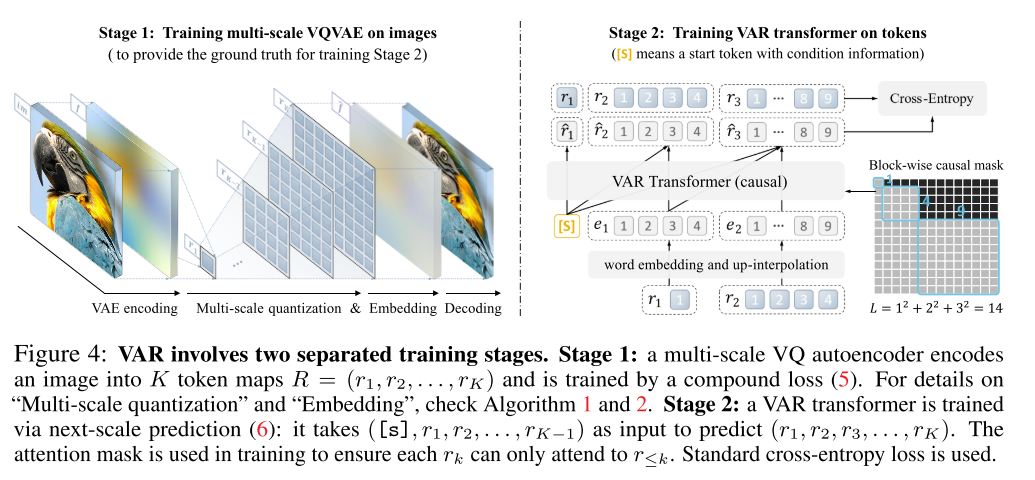
\includegraphics[width=0.8\textwidth]{./fig/VAR.png} 
    %\caption{这是一张示例图片} 
    \label{fig:VAR} 
\end{figure}

% \begin{algorithm}
% \caption{Multi-scale VQVAE Encoding}
% \label{alg:encoding}
% \begin{algorithmic}[1]
% \State Inputs: raw image $im$;
% \State Hyperparameters: steps $K$, resolutions $(h_k, w_k)$ for $k=1$;
% \State $f = E(im)$, $R = []$;
% \For{$k = 1$ to $K$}
%     \State $r_k = Q(\text{interpolate}(f, h_k, w_k))$;
%     \State $R = \text{queue\_push}(R, r_k)$;
%     \State $z_k = \text{lookup}(Z, r_k)$;
%     \State $z_k = \text{interpolate}(z_k, h_K, w_K)$;
%     \State $f = f - \phi_k(z_k)$;
% \EndFor
% \State \Return multi-scale tokens $R$;
% \end{algorithmic}
% \end{algorithm}

% \begin{algorithm}
% \caption{Multi-scale VQVAE Reconstruction}
% \label{alg:reconstruction}
% \begin{algorithmic}[1]
% \State Inputs: multi-scale token maps $R$;
% \State Hyperparameters: steps $K$, resolutions $(h_k, w_k)$ for $k=1$;
% \State $f = 0$;
% \For{$k = 1$ to $K$}
%     \State $r_k = \text{queue\_pop}(R)$;
%     \State $z_k = \text{lookup}(Z, r_k)$;
%     \State $z_k = \text{interpolate}(z_k, h_K, w_K)$;
%     \State $f = f + \phi_k(z_k)$;
% \EndFor
% \State $im = D(f)$;
% \State \Return reconstructed image $im$;
% \end{algorithmic}
% \end{algorithm}

\begin{figure}[htbp]
    \centering
    \begin{minipage}{0.45\textwidth}
        \centering
        \begin{algorithm}[H]
            \caption{Multi-scale VQVAE Encoding}
            \begin{algorithmic}[1]
                \Require raw image $im$; 
                \Require Hyperparameters: steps $K$, resolutions $(h_k, w_k)_{k=1}^K$;
                \State $f = \mathcal{E}(im)$, $R = []$;
                \For{$k = 1, \cdots, K$}
                    \State $r_k = \mathcal{Q}(\text{interpolate}(f, h_k, w_k))$;
                    \State $R = \text{queue\_push}(R, r_k)$;
                    \State $z_k = \text{lookup}(Z, r_k)$;
                    \State $z_k = \text{interpolate}(z_k, h_K, w_K)$;
                    \State $f = f - \phi_k(z_k)$;
                \EndFor
                \Ensure multi-scale tokens $R$;
            \end{algorithmic}
        \end{algorithm}
    \end{minipage}\hfill
    \begin{minipage}{0.45\textwidth}
        \centering
        \begin{algorithm}[H]
            \caption{Multi-scale VQVAE Reconstruction}
            \begin{algorithmic}[1]
                \Require multi-scale token maps $R$;
                \Require Hyperparameters: steps $K$, resolutions $(h_k, w_k)_{k=1}^K$;
                \State $\hat{f} = 0$;
                \For{$k = 1, \cdots, K$}
                    \State $r_k = \text{queue\_pop}(R)$;
                    \State $z_k = \text{lookup}(Z, r_k)$;
                    \State $z_k = \text{interpolate}(z_k, h_K, w_K)$;
                    \State $\hat{f} = \hat{f} + \phi_k(z_k)$;
                \EndFor
                \State $\hat{im} = \mathcal{D}(\hat{f})$;
                \Ensure reconstructed image $\hat{im}$;
            \end{algorithmic}
        \end{algorithm}
    \end{minipage}
    \caption{Algorithms for Multi-scale VQVAE Encoding and Reconstruction}
\end{figure}